\documentclass[letterpaper, twoside, 12pt]{book}
\usepackage{packet}


\begin{document}

\setcounter{chapter}{0}

\chapter{Chapter 12: Vectors and the Geometry of Space}

\setcounter{chapter}{12}

\section{Two and Three Dimensional Space}

\begin{definition}
  Let $\mathbb{R}$ be the collection of real numbers, let $\mathbb{R}^2$ be the
  collection of all \textbf{ordered pairs} of real numbers, and let $\mathbb{R}^3$
  be the collection of all \textbf{ordered triples} of real numbers.

  $\mathbb{R}$ is known as the \textbf{real line}, $\mathbb{R}^2$ is known
  as the \textbf{real plane} or the \textbf{$xy$-plane}, and $\mathbb{R}^3$
  is known as \textbf{real (3D) space} or \textbf{$xyz$-space}.
\end{definition}

\begin{center}
  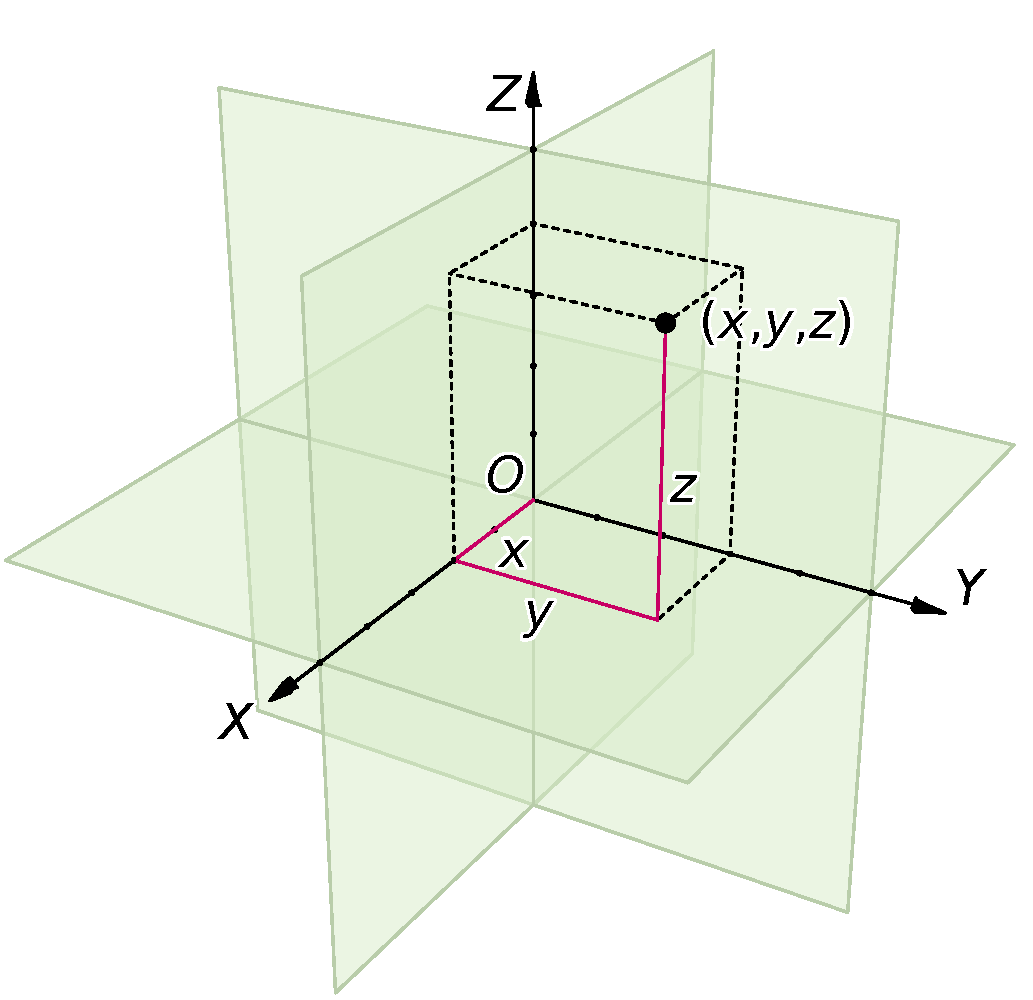
\includegraphics[width=0.5\textwidth]{assets/3dCoordinateSystem.pdf}
\end{center}

\begin{definition}
  The \textbf{distance} between two points $P=(x_1,y_1)$ and
  $Q=(x_2,y_2)$ in $\mathbb{R}^2$ is given by the formula
  \[
    d(P,Q) = \sqrt{(x_2-x_1)^2+(y_2-y_1)^2}
  \]

  The \textbf{distance} between two points $P=(x_1,y_1,z_1)$ and
  $Q=(x_2,y_2,z_2)$ in $\mathbb{R}^3$ is given by the formula
  \[
    d(P,Q) = \sqrt{(x_2-x_1)^2+(y_2-y_1)^2+(z_2-z_1)^2}
  \]
\end{definition}

          \begin{problem}
            Plot and find the distance between the points
            $(-2,6)$ and $(3,-6)$.
          \end{problem}

          \begin{solution}

          \end{solution}

          \begin{problem}
            Plot and find the distance between the points
            $(0,0,0)$ and $(4,2,4)$.
          \end{problem}

          \begin{solution}

          \end{solution}

          \begin{problem}
            Plot and find the distance between the points
            $(3,7,-2)$ and $(-1,7,1)$.
          \end{problem}

          \begin{solution}

          \end{solution}

          \begin{problem}
            Plot and find the distance between the points
            $(8,2,1)$ and $(4,-2,7)$.
          \end{problem}

          \begin{solution}

          \end{solution}





\begin{definition}
  \textbf{Simple lines} in $\mathbb{R}^2$ are given by the relations $x=a$,
  and $y=b$ for real numbers $a,b$.

  \textbf{Simple planes} in $\mathbb{R}^3$ are given by the relations $x=a$,
  $y=b$, $z=c$ for real numbers $a,b,c$.
\end{definition}

\begin{definition}
  A \textbf{circle} in $\mathbb{R}^2$ is the set of all points a fixed distance
  (called its \textbf{radius}) from a fixed point (called its \textbf{center}).
  For a center $(a,b)$ and radius $r$, the equation for a circle is
  \[
    (x-a)^2+(y-b)^2=r^2
  \]

  A \textbf{sphere} in $\mathbb{R}^3$ is the set of all points a fixed distance
  (called its \textbf{radius}) from a fixed point (called its \textbf{center}).
  For a center $(a,b,c)$ and radius $r$, the equation for a sphere is
  \[
    (x-a)^2+(y-b)^2+(z-c)^2=r^2
  \]
\end{definition}

          \begin{problem}
            Plot the curve $x=3$ in the $xy$-plane and the surface
            $x=3$ in $xyz$-space.
          \end{problem}

          \begin{solution}

          \end{solution}

          \begin{problem}
            Plot the curve $y=-1$ in the $xy$-plane and and the surface
            $y=-1$ in $xyz$-space.
          \end{problem}

          \begin{solution}

          \end{solution}

          \begin{problem}
            Plot the surface $z=0$ in $xyz$-space.
          \end{problem}

          \begin{solution}

          \end{solution}

          \begin{problem}
            Plot the curve $(x-2)^2+(y+1)^2=9$ in the $xy$-plane.
          \end{problem}

          \begin{solution}

          \end{solution}

          \begin{problem}
            Plot the surface $x^2+y^2+z^2=4$ in $xyz$-space.
          \end{problem}

          \begin{solution}

          \end{solution}

          \begin{problem}
            Plot the curve $x^2+(y-1)^2+z^2=1$ in $xyz$-space.
          \end{problem}

          \begin{solution}

          \end{solution}



\begin{suggestedHW}
Section $12.1$ numbers $4,$ $6,$ $7,$ $8,$ $10,$ $11,$ $12,$ $14,$ $15,$ $16$
\end{suggestedHW}



\section{Vectors}

\begin{definition}[Vector\index{Vector}]
  A \textbf{vector} $\harpvec v$ is a mathematical object that stores a
  \textbf{magnitude} (a nonnegative real number often thought of as length)
  and \textbf{direction}. Two vectors are \textbf{equal} if and only if they
  have the same magnitude and direction.
\end{definition}

\begin{definition}
  The \textbf{zero vector} $\harpvec0$ has zero magnitude and no direction.
  (This is the only vector without a direction.)
\end{definition}

\begin{definition}
  For a given point $P=(a,b)$ in $\mathbb{R}^2$, its \textbf{position vector}
  is given by $\harpvec{P}=\<a,b\>$: the vector from the origin $(0,0)$ to the
  point $P=(a,b)$.

  For a given point $P=(a,b,c)$ in $\mathbb{R}^3$, its \textbf{position vector}
  is given by $\harpvec{P}=\<a,b,c\>$: the vector from the origin $(0,0,0)$ to
  the point $P=(a,b,c)$.
\end{definition}

\begin{theorem}
  Two vectors are equal if and only if they share the same magnitude and
  direction as a common position vector.
\end{theorem}

\begin{definition}
  Since all vectors are equal to some position vector $\<a,b\>$ or $\<a,b,c\>$,
  we usually define vectors by a position vector written in this
  \textbf{component form}.
  Since the component form of a vector stores the same information as a point,
  we will use both interchangeably, that is, $\<a,b\>=(a,b)\in\mathbb{R}^2$ and
  $\<a,b,c\>=(a,b,c)\in\mathbb{R}^3$
  (although we usually sketch them differently).
\end{definition}

          \begin{problem}
            Plot the point $(1,3)$ and the position vector
            $\<1,3\>$ in the $xy$-plane.
          \end{problem}

          \begin{solution}

          \end{solution}

          \begin{problem}
            Plot the point $(-2,5)$ and the position vector
            $\<-2,5\>$ in the $xy$-plane.
          \end{problem}

          \begin{solution}

          \end{solution}

          \begin{problem}
            Plot the point $(1,1,-3)$ and the position vector
            $\<1,1,-3\>$ in $xyz$-space.
          \end{problem}

          \begin{solution}

          \end{solution}

          \begin{problem}
            Plot the point $(0,5,0)$ and the position vector
            $\<0,5,0\>$ in $xyz$-space.
          \end{problem}

          \begin{solution}

          \end{solution}





\begin{definition}
  Let $P = \left(x_1,y_1,z_1\right)$ and $Q = \left(x_2,y_2,z_2\right).$
  Then the vector with initial point $P$ and terminal point $Q$ is defined as
  \[
    \harpvec{PQ} = \threevec{x_2 - x_1}{y_2 - y_1}{z_2 - z_1}
  \]
\end{definition}

          \begin{problem}
            Plot $P=(1,3)$ and $Q=(-3,6)$ in the $xy$-plane.
            Then compute and plot the vector $\harpvec{PQ}$.
          \end{problem}

          \begin{solution}

          \end{solution}

          \begin{problem}
            Plot $P=(3,1)$ and $Q=(0,-2)$ in the $xy$-plane.
            Then compute and plot the vector $\harpvec{PQ}$.
          \end{problem}

          \begin{solution}

          \end{solution}

          \begin{problem}
            Plot $P=(1,1,1)$ and $Q=(-3,-1,3)$ in $xyz$-space.
            Then compute and plot the vector $\harpvec{PQ}$.
          \end{problem}

          \begin{solution}

          \end{solution}

          \begin{problem}
            Plot $P=(-2,0,3)$ and $Q=(1,3,-3)$ in $xyz$-space.
            Then compute and plot the vector $\harpvec{PQ}$.
          \end{problem}

          \begin{solution}

          \end{solution}



\begin{definition}
  The magnitude $|\harpvec{v}|$ of a vector $\harpvec{v}$ in $\mathbb{R}^2$ or
  $\mathbb{R}^3$ is the distance between its initial and terminal points.
\end{definition}

\begin{theorem}
  The magnitude of $\harpvec{v}=\<a,b\>$ is given by
    \[|\harpvec{v}|=\sqrt{a^2+b^2}\]

  The magnitude of $\harpvec{v}=\<a,b,c\>$ is given by
    \[|\harpvec{v}|=\sqrt{a^2+b^2+c^2}\]
\end{theorem}



          \begin{problem}
            Evaluate the magnitude of the position vector $\<5,5\>$.
          \end{problem}

          \begin{solution}

          \end{solution}

          \begin{problem}
            Evaluate the magnitude of the position vector $\<-4,3\>$.
          \end{problem}

          \begin{solution}

          \end{solution}

          \begin{problem}
            Evaluate the magnitude of the position vector $\<12,-5\>$.
          \end{problem}

          \begin{solution}

          \end{solution}

          \begin{problem}
            Evaluate the magnitude of the position vector $\<3,1,-2\>$.
          \end{problem}

          \begin{solution}

          \end{solution}

          \begin{problem}
            Evaluate the magnitude of the position vector $\<4,-2,-4\>$.
          \end{problem}

          \begin{solution}

          \end{solution}

          \begin{problem}
            Evaluate the magnitude of the position vector $\<8,0,-6\>$.
          \end{problem}

          \begin{solution}

          \end{solution}



\begin{definition}
  \textbf{Vector addition} is defined component-wise as follows for
  $\mathbb{R}^2$ and $\mathbb{R}^3$
  \[
    \harpvec{u}+\harpvec{v}
      =
    \<u_1,u_2\>+\<v_1,v_2\>
      =
    \<u_1+v_1,u_2+v_2\>
  \]
  \[
    \harpvec{u}+\harpvec{v}
      =
    \<u_1,u_2,u_3\>+\<v_1,v_2,v_3\>
      =
    \<u_1+v_1,u_2+v_2,u_3+v_3\>
  \]
\end{definition}

\begin{definition}
  A \textbf{scalar} is simply a real number by itself
  (as opposed to a vector of real numbers).
\end{definition}

\begin{definition}
  \textbf{Scalar multiplication of a vector} is defined component-wise as
  follows for $\mathbb{R}^2$ and $\mathbb{R}^3$:
  \[
    k\harpvec{u}
      =
    k\<u_1,u_2\>
      =
    \<ku_1,ku_2\>
  \]
  \[
    k\harpvec{u}
      =
    k\<u_1,u_2,u_3\>
      =
    \<ku_1,ku_2,ku_3\>
  \]
\end{definition}



          \begin{problem}
            Compute and plot $\harpvec{u}=\<1,-3\>$, $\harpvec{v}=\<3,1\>$
            and $\harpvec{u}+\harpvec{v}$ in the $xy$-plane.
          \end{problem}

          \begin{solution}

          \end{solution}

          \begin{problem}
            Compute and plot $\harpvec{u}=\<2,0,1\>$, $\harpvec{v}=\<-2,4,2\>$
            and $\harpvec{u}+\harpvec{v}$ in $xyz$-space.
          \end{problem}

          \begin{solution}

          \end{solution}

          \begin{problem}
            Compute and plot $\harpvec{u}=\<8,-2\>$ and
            $\frac{1}{2}\harpvec{u}$ in the $xy$-plane.
          \end{problem}

          \begin{solution}

          \end{solution}

          \begin{problem}
            Compute and plot $\harpvec{u}=\<5,3,-1\>$ and
            $3\harpvec{u}$ in $xyz$-space.
          \end{problem}

          \begin{solution}

          \end{solution}



\begin{definition}
  A vector $\harpvec{v}$ is a \textbf{unit vector} if $|\harpvec v|=1$.
\end{definition}

\begin{theorem}
  For any non-zero vector $\harpvec{v}$, the vector
  \[
    \frac{1}{|\harpvec v|}\harpvec{v} = \frac{\harpvec v}{|\harpvec v|}
  \]
  is a unit vector.
\end{theorem}

\begin{definition}
  The \textbf{direction} of a vector $\harpvec v$ is the unit vector
  $\frac{\harpvec v}{|\harpvec v|}$.
\end{definition}

\begin{theorem}
  Any vector $\harpvec v$ is the scalar product of its magnitude and direction:
  \[
    \harpvec v = |\harpvec v|\frac{\harpvec v}{|\harpvec v|}
  \]
\end{theorem}



          \begin{problem}
            Rewrite $\<5,5\>$ as the scalar product of its magnitude and
            direction.
          \end{problem}

          \begin{solution}

          \end{solution}

          \begin{problem}
            Rewrite $\<-4,3\>$ as the scalar product of its magnitude and
            direction.
          \end{problem}

          \begin{solution}

          \end{solution}

          \begin{problem}
            Rewrite $\<12,-5\>$ as the scalar product of its magnitude and
            direction.
          \end{problem}

          \begin{solution}

          \end{solution}

          \begin{problem}
            Rewrite $\<3,1,-2\>$ as the scalar product of its magnitude and
            direction.
          \end{problem}

          \begin{solution}

          \end{solution}

          \begin{problem}
            Rewrite $\<4,-2,-4\>$ as the scalar product of its magnitude and
            direction.
          \end{problem}

          \begin{solution}

          \end{solution}

          \begin{problem}
            Rewrite $\<8,0,-6\>$ as the scalar product of its magnitude and
            direction.
          \end{problem}

          \begin{solution}

          \end{solution}



\begin{definition}
The \textbf{standard unit vectors} in $\mathbb{R}^2$ are
$\veci=\<1,0\>$ and $\vecj=\<0,1\>$, and any vector in $\mathbb{R}^2$
can be expressed in \textbf{standard unit vector form}:
  \[\<a,b\>=a\veci+b\vecj\]

The \textbf{standard unit vectors} in $\mathbb{R}^3$ are
$\veci=\<1,0,0\>$, $\vecj=\<0,1,0\>$, and $\veck=\<0,0,1\>$, and any vector in
$\mathbb{R}^3$ can be expressed in \textbf{standard unit vector form}:
  \[\<a,b,c\>=a\veci+b\vecj+c\veck\]
\end{definition}

\begin{remark}
  Since the $xy$-plane is the the plane $z=0$ in $xyz$-space, we say the
  points and vectors $(a,b)=(a,b,0)=\<a,b\>=\<a,b,0\>=a\veci+b\vecj+0\veck$
  are all equal.
\end{remark}



          \begin{problem}
            Rewrite $\<5,5\>$ in standard unit vector form.
          \end{problem}

          \begin{solution}

          \end{solution}

          \begin{problem}
            Rewrite $\<-4,3\>$ in standard unit vector form.
          \end{problem}

          \begin{solution}

          \end{solution}

          \begin{problem}
            Rewrite $\<3,1,-2\>$ in standard unit vector form.
          \end{problem}

          \begin{solution}

          \end{solution}

          \begin{problem}
            Rewrite $\<8,0,-6\>$ in standard unit vector form.
          \end{problem}

          \begin{solution}

          \end{solution}



\begin{theorem}
The following properties hold for any two vectors $\harpvec{u}$, $\harpvec{v}$
and scalars $a$, $b$.
  \begin{itemize}
  \item $\harpvec{u}+\harpvec{v} = \harpvec{v}+\harpvec{u}$
  \item $(\harpvec{u}+\harpvec{v})+\harpvec{w} = \harpvec{u}+(\harpvec{v}+\harpvec{w})$
  \item $\harpvec{u}+\harpvec{0} = \harpvec{u}$
  \item $\harpvec{u}+(-\harpvec{u}) = \harpvec{0}$
  \item $0\harpvec{u} = \harpvec{0}$
  \item $1\harpvec{u} = \harpvec{u}$
  \item $a(b\harpvec{u}) = (ab)\harpvec{u}$
  \item $a(\harpvec{u} + \harpvec{v}) = a\harpvec{u} + a\harpvec{v}$
  \item $(a+b)\harpvec{u} = a\harpvec{u} + b\harpvec{u}$
  \end{itemize}
\end{theorem}

\begin{definition}
  \textbf{Vector subtraction} is defined as the addition of a negative:
  \[
    \harpvec{u}-\harpvec{v}
      =
    \harpvec{u}+(-\harpvec{v})
      =
    \<u_1-v_1,u_2-v_2\>
  \]
  \[
    \harpvec{u}-\harpvec{v}
      =
    \harpvec{u}+(-\harpvec{v})
      =
    \<u_1-v_1,u_2-v_2,u_3-v_3\>
  \]
\end{definition}

\begin{suggestedHW}
Section $12.2$ numbers $3,$ $5,$ $13,$ $14,$ $15,$ $19,$ $21,$ $24,$ $26$
\end{suggestedHW}



\section{The Dot Product}

\begin{definition}
  Let $\theta$ be the angle between two non-zero vectors $\harpvec{u}$, $\harpvec{v}$.
  The \textbf{dot product} $\harpvec{u}\cdot\harpvec{v}$ is the product of their
  lengths when projected into the same direction, obtained by this formula:
  \[
    \harpvec{u} \cdot \harpvec{v} = |\harpvec{u}||\harpvec{v}|\cos \theta
  \]
\end{definition}

\begin{definition}
  The dot product with a zero vector is always zero:
  \[\harpvec{v}\cdot\harpvec{0}=\harpvec{0}\cdot\harpvec{v}=0\]
\end{definition}

\begin{theorem}
By the Law of Cosines:
  \[
    \harpvec{u} \cdot \harpvec{v}
      =
    \<u_1,u_2\>\cdot\<v_1,v_2\>
      =
    u_1v_1 + u_2v_2
  \]
  \[
    \harpvec{u} \cdot \harpvec{v}
      =
    \<u_1,u_2,u_3\>\cdot\<v_1,v_2,v_3\>
      =
    u_1v_1 + u_2v_2 + u_3v_3
  \]
\end{theorem}

\begin{definition}
  Two vectors $\harpvec{u},\harpvec{v}$ are \textbf{orthogonal} if
  $\harpvec{u} \cdot \harpvec{v} = 0$.
\end{definition}

\begin{theorem}
  Two non-zero vectors are orthogonal if the angle $\theta$ between them
  is $\frac{\pi}{2}$ radians.
\end{theorem}

\begin{theorem}
The following properties hold for any three vectors $\harpvec{u}$, $\harpvec{v}$,
$\harpvec{w}$ and scalar $c$.
  \begin{itemize}
  \item $\harpvec{u} \cdot \harpvec{v} = \harpvec{v}\cdot\harpvec{u}$
  \item $(c\harpvec{u})\cdot \harpvec{v} = \harpvec{u} \cdot (c\harpvec{v}) = c(\harpvec{u} \cdot \harpvec{v})$
  \item $\harpvec{u} \cdot (\harpvec{v} + \harpvec{w}) = \harpvec{u}\cdot\harpvec{v} + \harpvec{u}\cdot \harpvec{w}$
  \item $\harpvec{u} \cdot \harpvec{u} = |\harpvec{u}|^2$
  \end{itemize}
\end{theorem}

          \begin{problem}
            Compute the angle between the vectors
            $\harpvec{u}=\<4,-3\>$ and $\harpvec{v}=\<5,12\>$.
          \end{problem}

          \begin{solution}

          \end{solution}

          \begin{problem}
            Compute the angle between the vectors
            $\harpvec{u}=\<1,4,2\>$ and $\harpvec{v}=\<4,1,-2\>$.
          \end{problem}

          \begin{solution}

          \end{solution}

          \begin{problem}
            Compute the angle between the vectors
            $\harpvec{u}=\<0,5,-11\>$ and $\harpvec{v}=\<2,0,0\>$.
          \end{problem}

          \begin{solution}

          \end{solution}



\begin{definition}
The work $W$ done by a force vector $\harpvec{F}$ over a displacement
vector $\harpvec{D}$ is given by
\[
  W = \harpvec{F} \cdot \harpvec{D}
    =
  |\harpvec{F}||\harpvec{D}|\cos \theta
\]
\end{definition}

\begin{suggestedHW}
Section $12.3$ numbers
$3,$ $5,$ $6,$ $7,$ $8,$ $9,$ $10,$ $11,$ $15,$ $17,$
$21,$ $27,$ $41,$ $42,$ $44$
\end{suggestedHW}





\section{The Cross Product}

\begin{definition}
  For any two non-parallel vectors $\harpvec{u}$, $\harpvec{v}$ in $\mathbb R^3$,
  the \textbf{Right-Hand Rule} gives a specific direction orthogonal to both:
  position $\harpvec{u}$ with your right thumb and $\harpvec{v}$ with your
  right index finger, and let your middle finger extend orthogonal to both
  to give this direction.
\end{definition}

\begin{definition}
  Let $\theta$ be the angle between two non-zero vectors $\harpvec{u}$,
  $\harpvec{v}$ in $\mathbb{R}^3$, and let $\harpvec{n}$ be the direction
  given by the Right-Hand Rule.
  The \textbf{cross product} $\harpvec{u}\times\harpvec{v}$ is the vector
  orthogonal to both which follows the Right-Hand Rule and has magnitude
  equal to the area of the parallelogram formed from both.
  \[
    \harpvec{u}\times\harpvec{v}
      =
    (|\harpvec{u}||\harpvec{v}|\sin\theta)\harpvec{n}
  \]
  \[
    |\harpvec{u}\times\harpvec{v}|
      =
    |\harpvec{u}||\harpvec{v}|\sin\theta
  \]
\end{definition}

\begin{definition}
  The cross product with a zero vector is always the zero vector:
  \[\harpvec{v}\times\harpvec{0}=\harpvec{0}\times\harpvec{v}=\harpvec{0}\]
\end{definition}

\begin{theorem}
  The following properties hold for any three vectors $\harpvec{u}$, $\harpvec{v}$,
  $\harpvec{w}$ and scalars $a$,$b$.
  \begin{itemize}
  \item $(a\harpvec{u}) \times (b\harpvec{v}) = (ab)(\harpvec{u} \times \harpvec{v})$
  \item
    $\harpvec{u} \times (\harpvec{v} + \harpvec{w}) =
    \harpvec{u} \times \harpvec{v} + \harpvec{u} \times \harpvec{w}$
  \item
    $(\harpvec{v} + \harpvec{w}) \times \harpvec{u} =
    \harpvec{v} \times \harpvec{u} + \harpvec{w} \times \harpvec{u}$
  \item $\harpvec{v} \times \harpvec{u} = -(\harpvec{u} \times \harpvec{v})$
  \end{itemize}
\end{theorem}

\begin{definition}
  Two vectors $\harpvec{u},\harpvec{v}$ are \textbf{parallel} if
  $\harpvec{u} \times \harpvec{v} = 0$.
\end{definition}

\begin{theorem}
  Two non-zero vectors are parallel if the angle $\theta$ between them
  is $0$ or $\pi$ radians.
\end{theorem}

\begin{definition}
  The cross products of the standard unit vectors are given as follows:
  \begin{itemize}
    \item $\veci \times \vecj = \veck$
    \item $\vecj \times \veck = \veci$
    \item $\veck \times \veci = \vecj$
  \end{itemize}
\end{definition}

\begin{definition}
  A \textbf{determinant} is a short hand for writing certain commonly
  occuring algebraic expressions:
    \[
      \begin{array}{|c c|}
      a_1 & a_2 \\
      b_1 & b_2 \\
      \end{array}
        =
      a_1b_2 - a_2b_1
    \]
    \[
      \begin{array}{|c c c|}
      a_1 & a_2 & a_3 \\
      b_1 & b_2 & b_3 \\
      c_1 & c_2 & c_3 \\
      \end{array}
        =
      a_1 \,
      \begin{array}{|c c|}
      b_2 & b_3 \\
      c_2 & c_3 \\
      \end{array}
        -
      a_2 \,
      \begin{array}{|c c|}
      b_1 & b_3 \\
      c_1 & c_3 \\
      \end{array}
        +
      a_3 \,
      \begin{array}{|c c|}
      b_1 & b_2 \\
      c_1 & c_2 \\
      \end{array}
    \]
\end{definition}



\begin{theorem}
  By breaking up $\harpvec{u}$, $\harpvec{v}$ into standard unit vectors:
  \[
  \harpvec{u} \times \harpvec{v}
    =
  \begin{array}{|c c c|}
  \veci & \vecj & \veck \\
  u_1 & u_2 & u_3 \\
  v_1 & v_2 & v_3 \\
  \end{array}
    =
  \left\<
    \begin{array}{|c c|}
    u_2 & u_3 \\
    v_2 & v_3 \\
    \end{array}
      \,,-\,
    \begin{array}{|c c|}
    u_1 & u_3 \\
    v_1 & v_3 \\
    \end{array}
      \,,\,
    \begin{array}{|c c|}
    u_1 & u_2 \\
    v_1 & v_2 \\
    \end{array}
  \right\>
  \]
\end{theorem}

          \begin{problem}
            Compute a nonzero vector normal to both $\harpvec{u}=\<4,-3,0\>$
            and $\harpvec{v}=\<2,6,-3\>$.
          \end{problem}

          \begin{solution}

          \end{solution}

          \begin{problem}
            Compute a nonzero vector normal to both $\harpvec{u}=\<1,4,2\>$
            and $\harpvec{v}=\<4,1,-2\>$.
          \end{problem}

          \begin{solution}

          \end{solution}

          \begin{problem}
            Compute a nonzero vector normal to both $\harpvec{u}=\<0,5,-11\>$
            and $\harpvec{v}=\<2,0,0\>$.
          \end{problem}

          \begin{solution}

          \end{solution}



\begin{definition}
  The torque $\tau$ done by a force vector $\harpvec{F}$ on an arm given by
  $\harpvec{D}$ is given by
  \[
    \tau = |\harpvec{F} \times \harpvec{D}|
      =
    |\harpvec{F}||\harpvec{D}|\sin \theta
  \]
\end{definition}

\begin{theorem}
  The volume of a parallelpiped determined by the vectors
  $\harpvec{u}$, $\harpvec{v}$, $\harpvec{w}$, is given by
  the \textbf{triple scalar product}
    \[
      (\harpvec{u}\times\harpvec{v})\cdot\harpvec{w} =
      \begin{array}{|c c c|}
      u_1 & u_2 & u_3 \\
      v_1 & v_2 & v_3 \\
      w_1 & w_2 & w_3 \\
      \end{array}
    \]
\end{theorem}

\begin{suggestedHW}
  Section $12.4$ numbers $1 - 3,$ $17,$ $19,$ $28,$ $29,$ $33,$ $35$
\end{suggestedHW}



\section{Lines and Planes in Space}

\begin{theorem}
  Let $L$ be the line in $\mathbb R^2$ normal to the vector $\harpvec N=\<A,B\>$
  and passing through the point $P_0=(x_0,y_0)$. Then every point $P=(x,y)$
  on the line $L$ must satisfy the following equations:
  \[
    \harpvec N \cdot \harpvec{P_0P} = 0
  \]
  \[
    A(x-x_0) + B(y-y_0) = 0
  \]

  Let $M$ be the plane in $\mathbb R^3$ normal to the vector $\harpvec N=\<A,B,C\>$
  and passing through the point $P_0=(x_0,y_0,z_0)$. Then every point $P=(x,y,z)$
  on the plane $M$ must satisfy the following equations:
  \[
    \harpvec N \cdot \harpvec{P_0P} = 0
  \]
  \[
    A(x-x_0) + B(y-y_0) + C(z-z_0) = 0
  \]
\end{theorem}

          \begin{problem}
            Find an equation for the line passing through $(1,-2)$ and parallel
            to the line with equation $2x-y=3$. Then plot both lines.
          \end{problem}

          \begin{solution}

          \end{solution}

          \begin{problem}
            Find an equation for the plane passing through $(1,3,-2)$ and
            normal to the vector $\<3,0,1\>$. Then plot the plane and vector.
          \end{problem}

          \begin{solution}

          \end{solution}

          \begin{problem}
            Find an equation for the plane passing through $(-2,0,4)$,
            $(1,3,3)$, and $(0,0,2)$. Then plot the plane and points.
          \end{problem}

          \begin{solution}

          \end{solution}



\begin{definition}
  \textbf{Parametric equations} $x(t),y(t)$
  for a curve in $\mathbb R^2$ assign a point $(x(t),y(t))$ of the curve
  to each value of $t$.

  \textbf{Parametric equations} $x(t),y(t),z(t)$
  for a curve in $\mathbb R^3$ assign a point $(x(t),y(t),z(t))$ of the curve
  to each value of $t$.
\end{definition}



          \begin{problem}
            Sketch the curve given by the parametric equations
            $x(t)=t$ and $y(t)=t^2$.
          \end{problem}

          \begin{solution}

          \end{solution}

          \begin{problem}
            Sketch the curve given by the parametric equations
            $x(t)=\sin t$ and $y(t)=\frac{t}{\pi}$.
          \end{problem}

          \begin{solution}

          \end{solution}

          \begin{problem}
            Sketch the curve given by the parametric equations
            $x(t)=1-t$, $y(t)=3t$, and $z(t)=2t-3$.
          \end{problem}

          \begin{solution}

          \end{solution}

          \begin{problem}
            Sketch the curve given by the parametric equations
            $x(t)=-t^2$, $y(t)=2$, and $z(t)=t$.
          \end{problem}

          \begin{solution}

          \end{solution}



\begin{theorem}
  Let $L$ be the line in $\mathbb R^2$ parallel to the vector $\harpvec v=\<a,b\>$
  and passing through the point $P_0=(x_0,y_0)$. Then every point $P=(x,y)$
  on the line $L$ must satisfy the following vector equation for some $t$:
  \[
    \harpvec{P} = \harpvec{v}t + \harpvec{P_0}
  \]
  Thus the line is given by the parametric equations
  \[
    x(t) = at + x_0
  \]
  \[
    y(t) = bt + y_0
  \]

  Let $L$ be the line in $\mathbb R^3$ parallel to the vector $\harpvec v=\<a,b,c\>$
  and passing through the point $P_0=(x_0,y_0,z_0)$. Then every point $P=(x,y,z)$
  on the line $L$ must satisfy the following vector equation for some $t$:
  \[
    \harpvec{P} = \harpvec{v}t + \harpvec{P_0}
  \]
  Thus the line is given by the parametric equations
  \[
    x(t) = at + x_0
  \]
  \[
    y(t) = bt + y_0
  \]
  \[
    z(t) = ct + z_0
  \]
\end{theorem}



          \begin{problem}
            Find parametric equations for the line with equation $y=-3x+1$
            in the $xy$ plane. Then plot the line.
          \end{problem}

          \begin{solution}

          \end{solution}

          \begin{problem}
            Find parametric equations for the line passing through $(1,3,-2)$
            and parallel to $\<3,0,1\>$ in $xyz$ space. Then plot the point,
            vector, and line.
          \end{problem}

          \begin{solution}

          \end{solution}

          \begin{problem}
            Find parametric equations for the line normal to the plane with
            equation $x+y+2z=4$ and passing through $(1,1,1)$ in $xyz$ space.
            Then plot the point, plane, and line.
          \end{problem}



\begin{suggestedHW}
  Section $12.5$ numbers $3,$ $4,$ $6,$ $7,$ $17,$ $19,$ $24,$ $27,$ $31,$ $32$
\end{suggestedHW}




\section{Cylinders and Quadratic Surfaces}

\begin{definition}
  A \textbf{cylindrical surface} is a 3D surface given by an
  equation of two variables.
\end{definition}

          \begin{problem}
            Plot the curve $y=x^2$ in the $xy$-plane and the
            cylindrical surface $y=x^2$ in $xyz$-space.
          \end{problem}

          \begin{solution}

          \end{solution}

          \begin{problem}
            Plot the curve $y=\sin z$ in the $yz$-plane and the
            cylindrical surface $y=\sin z$ in $xyz$-space.
          \end{problem}

          \begin{solution}

          \end{solution}

          \begin{problem}
            Plot the curve $z=e^x$ in the $xz$-plane and the
            cylindrical surface $z=e^x$ in $xyz$-space.
          \end{problem}

          \begin{solution}

          \end{solution}

\begin{definition}
  A \textbf{trace} of an equation of $x,y,z$ is obtained by substituting
  a constant for one of the variables.
\end{definition}

\begin{definition}
  A \textbf{quadric surface} is a surface defined by a second
  degree equation of $x,y,z$.
\end{definition}

\begin{remark}
  Many surfaces may be identified and sketched by using the traces
  $x=0$, $y=0$, and $z=0$.
\end{remark}

\begin{definition}
  An \textbf{ellipsoid} is a quadric surface with these main traces:
    \begin{itemize}
    \item Three ellipses (with parallel ellipses)
    \end{itemize}
\end{definition}

\begin{definition}
  An \textbf{elliptical cone} is a quadric surface with these main traces:
    \begin{itemize}
    \item Two double-lines (with parallel hyperbolas)
    \item One point (with parallel ellipses)
    \end{itemize}
\end{definition}

\begin{definition}
  An \textbf{elliptical paraboloid} is a quadric surface with these main traces:
    \begin{itemize}
    \item Two parabolas (with parallel parabolas)
    \item One point (with parallel ellipses)
    \end{itemize}
\end{definition}

\begin{definition}
  A \textbf{hyperbolic paraboloid} is a quadric surface with these traces:
    \begin{itemize}
    \item Two parabolas (with parallel parabolas)
    \item One double line (with parallel hyperbolas)
    \end{itemize}
\end{definition}

\begin{definition}
  A \textbf{hyperboloid of one sheet} is a quadric surface with these traces:
    \begin{itemize}
    \item Two hyperbolas (with parallel hyperbolas)
    \item One ellipsis (with parallel ellipses)
    \end{itemize}
\end{definition}

\begin{definition}
  A \textbf{hyperboloid of two sheets} is a quadric surface with these traces:
    \begin{itemize}
    \item Two hyperbolas (with parallel hyperbolas)
    \item One empty trace (with parallel ellipses)
    \end{itemize}
\end{definition}

          \begin{problem}
            Plot $x^2-y=-z^2$ and its traces in the planes $x=0$, $y=0$,
            and $z=0$.
            Name the quadric surface.
          \end{problem}

          \begin{solution}

          \end{solution}

          \begin{problem}
            Plot $y^2+z^2=4-4x^2$ and its traces in the planes $x=0$, $y=0$,
            and $z=0$.
            Name the quadric surface.
          \end{problem}

          \begin{solution}

          \end{solution}

          \begin{problem}
            Plot $z^2-9y^2=x^2$ and its traces in the planes $x=0$, $y=0$,
            and $z=0$.
            Name the quadric surface.
          \end{problem}

          \begin{solution}

          \end{solution}

          \begin{problem}
            Plot $y^2-z^2=4-4x^2$ and its traces in the planes $x=0$, $y=0$,
            and $z=0$.
            Name the quadric surface.
          \end{problem}

          \begin{solution}

          \end{solution}

          \begin{problem}
            Plot $4x^2-y^2-4z^2=16$ and its traces in the planes $x=0$, $y=0$,
            and $z=0$.
            Name the quadric surface.
          \end{problem}

          \begin{solution}

          \end{solution}

          \begin{problem}
            Plot $z=y^2-4x^2$ and its traces in the planes $x=0$, $y=0$,
            and $z=0$.
            Name the quadric surface.
          \end{problem}

          \begin{solution}

          \end{solution}


\end{document}